\section{User Interface}\label{sec:ui}

Since this work should be valuable to (German) tax offices, a basic user interface is provided.
However, the focus of this work is on the methods and not on the user interface.
The user interface is divided into two parts, the frontend and the backend.

\subsection{Backend}\label{subsec:backend}

% this work: endpoints
The framework used for the backend is \flask{}.
In this work, only the \texttt{GET} method is used.
There are multiple endpoints, which are used to retrieve data from the server:

\begin{itemize}
    \item \label{pt:docs}Documents: 
        Returns a list of documents, which best match the query.
        The query can be of type \texttt{match\_all}, which returns all documents in the database, 
        or a fuzzy full-text query, 
        or a \ac{knn} query on a certain field of the database.
        Moreover, the number and start index of the results returned can be specified.

    \item \label{pt:doc}Document: 
        Returns the document with the specified \texttt{id}.

    \item \label{pt:pdf}\ac{pdf}: 
        Returns the path to a \ac{pdf} file.
        In order to access the path information a query for a document with the specified \texttt{id} is performed.
    
    \item \label{pt:wordcloud}WordCloud: 
        Returns the bytes of a WordCloud image. 
        Depending on additional parameters, the WordCloud is either generated from one document or 
        the most similar documents to the query field, identified by \ac{knn}.

    \item \label{pt:termfrequency}\textcolor{red}{Term Frequency}
\end{itemize}

In order to test the endpoints during development, swagger documentation for every endpoint is provided.





\subsection{Frontend}\label{subsec:frontend}

The framework used for the frontend is \angular{}.
There are two main components, which are used to display the data:

\begin{itemize}
    \item \label{pt:home}Home: 
        The home component is used to display the results of a query.
        It consists of a search bar, which is used to enter the text query, and a list of results.
        If no text query is entered the first documents of the database, i.e. the result of a \texttt{match\_all} query, are displayed.
        The search component is shown in \autoref{fig:home_comp}.

    \item \label{pt:detail}Detail: 
        The detail component is used to display the details of a document.
        It consists of a card, which contains the title, authors, and abstract of the document.
        Moreover, the WordCloud of the document is displayed.
        The WordCloud is generated from the abstract of the document.
        The detail component is shown in \autoref{fig:detail_comp}.
\end{itemize}

\textcolor{red}{TODO: describe visualizations}


\begin{figure}[htp] % htp = hier (h), top (t), oder auf einer eigenen Seite (p).
    \centering
    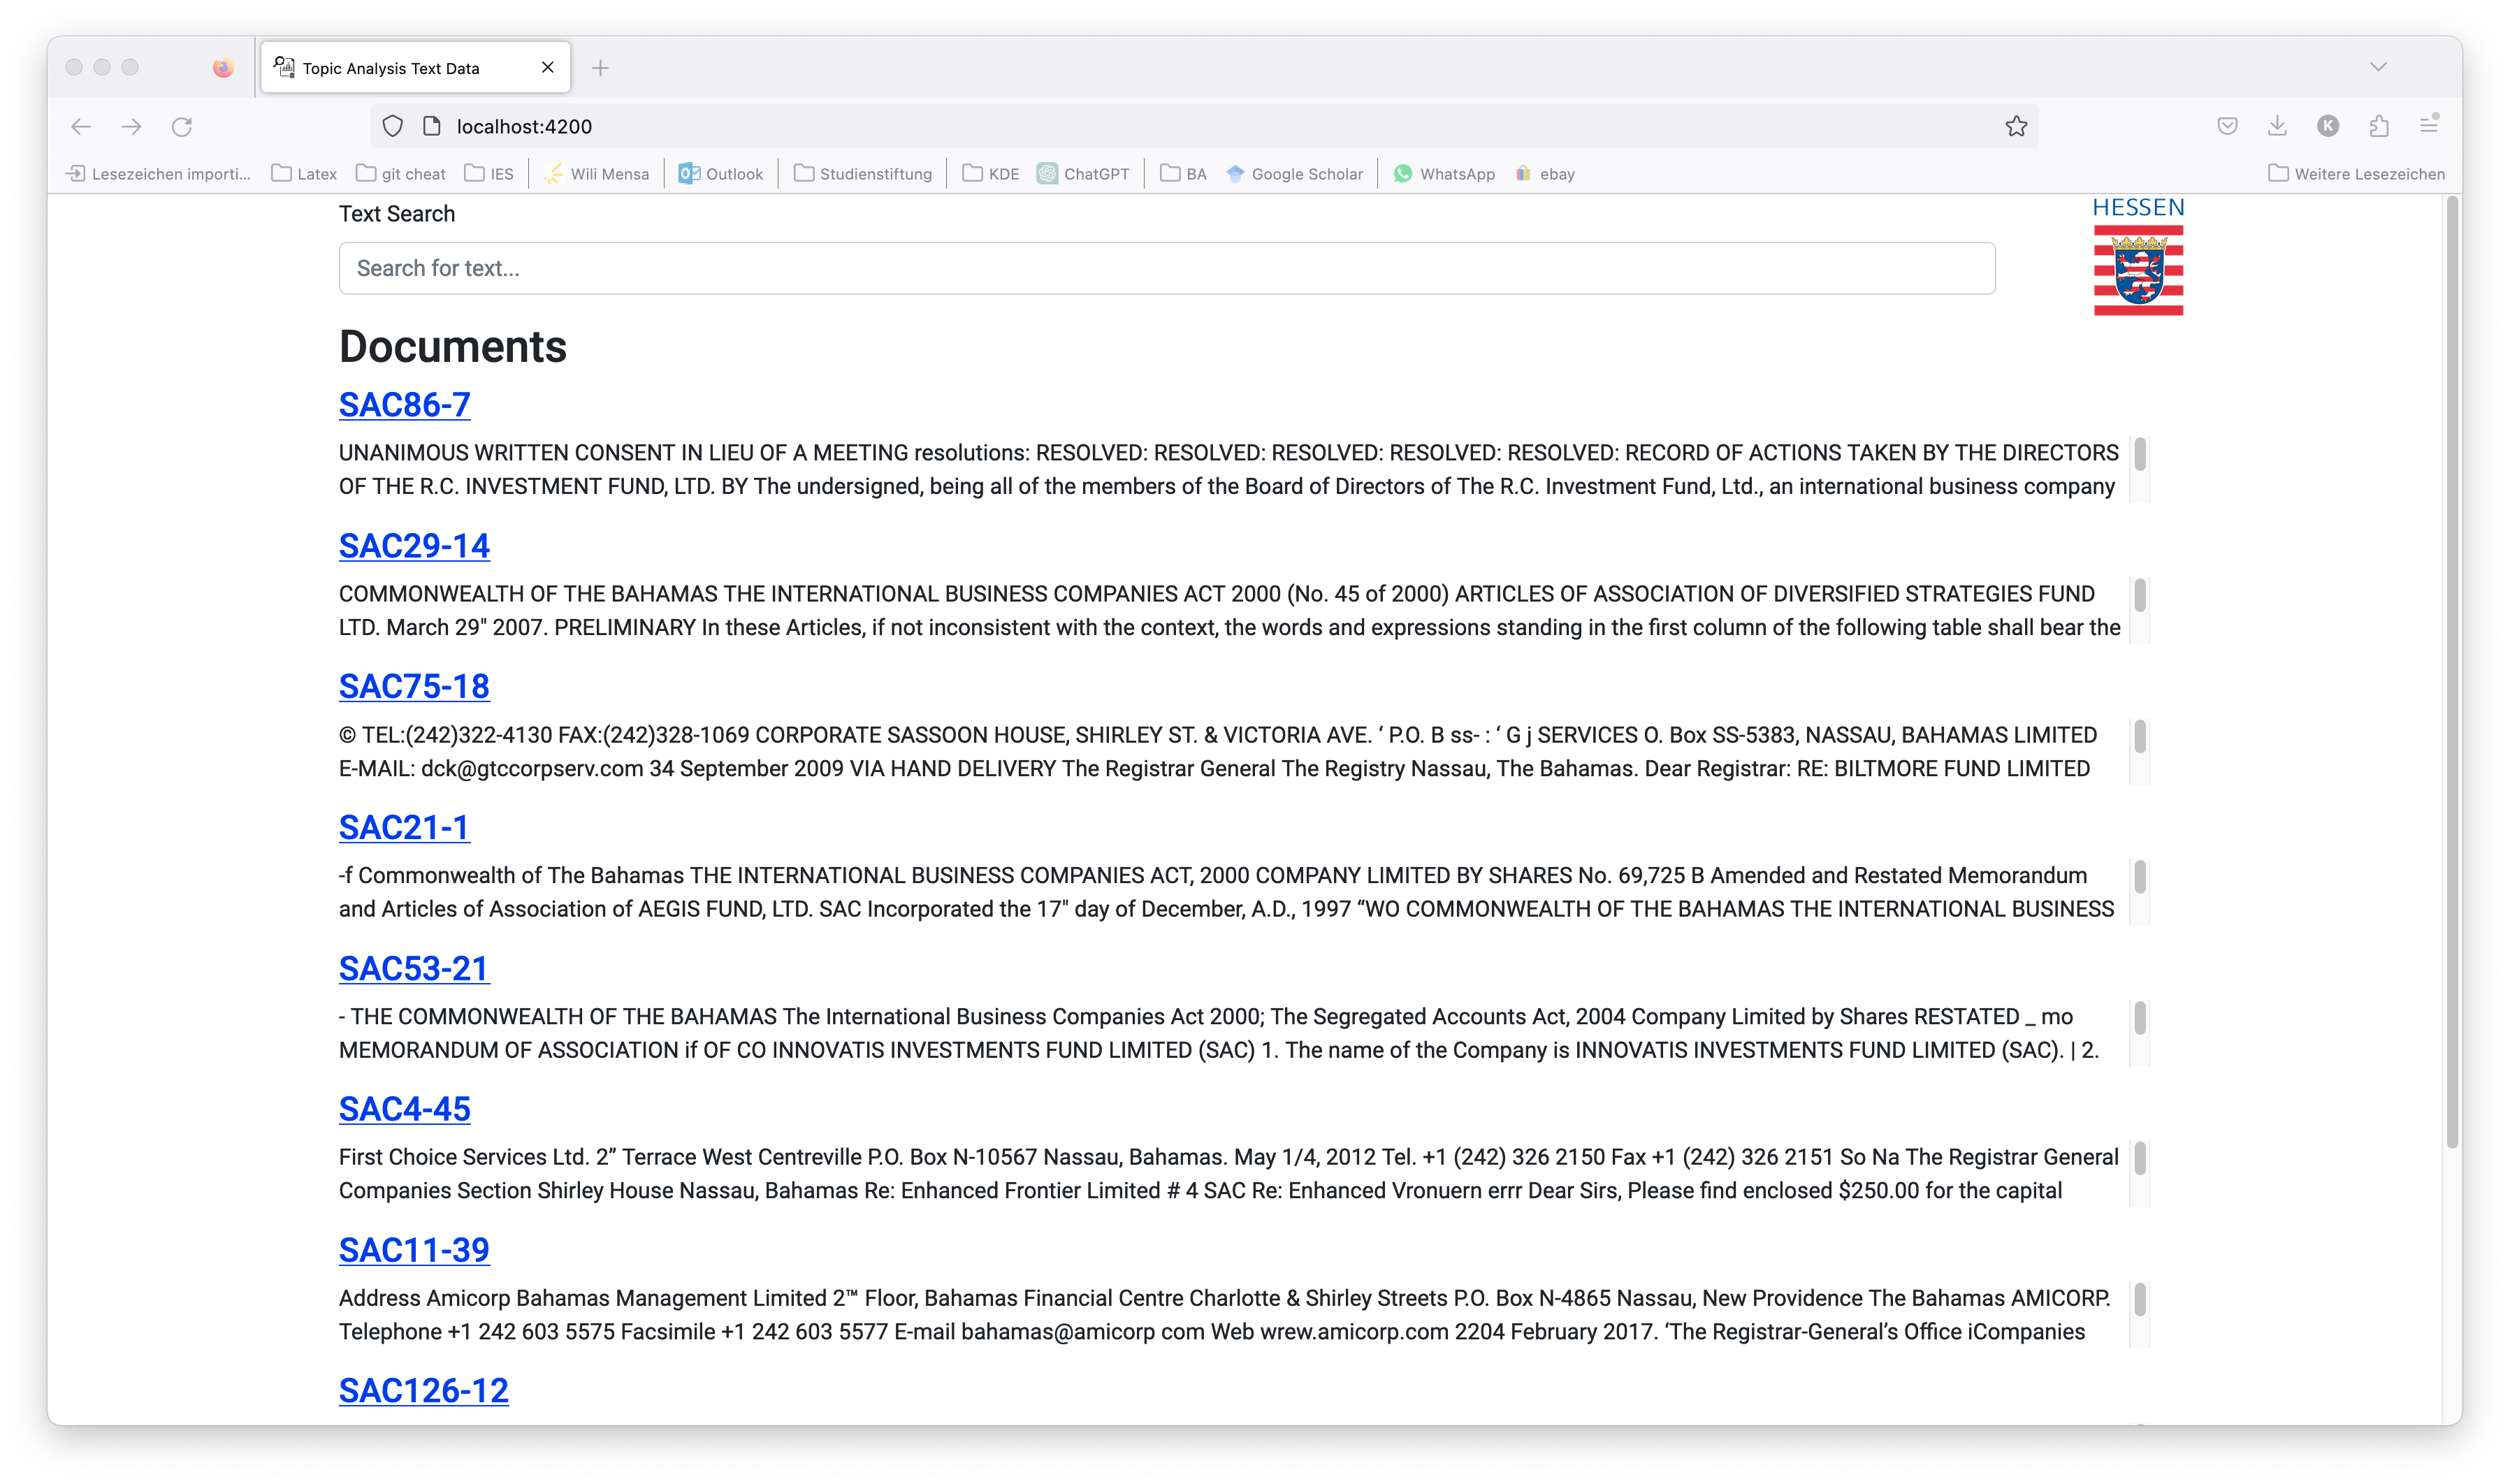
\includegraphics[width=0.6\textwidth]{images/UI/Home_component.png}
    \caption{Home component of the frontend.
    The search bar is used to enter the text query.
    The results of the query are displayed below the search bar.
    }
    \label{fig:home_comp}
\end{figure}


\begin{figure}[htp] % htp = hier (h), top (t), oder auf einer eigenen Seite (p).
    \centering
    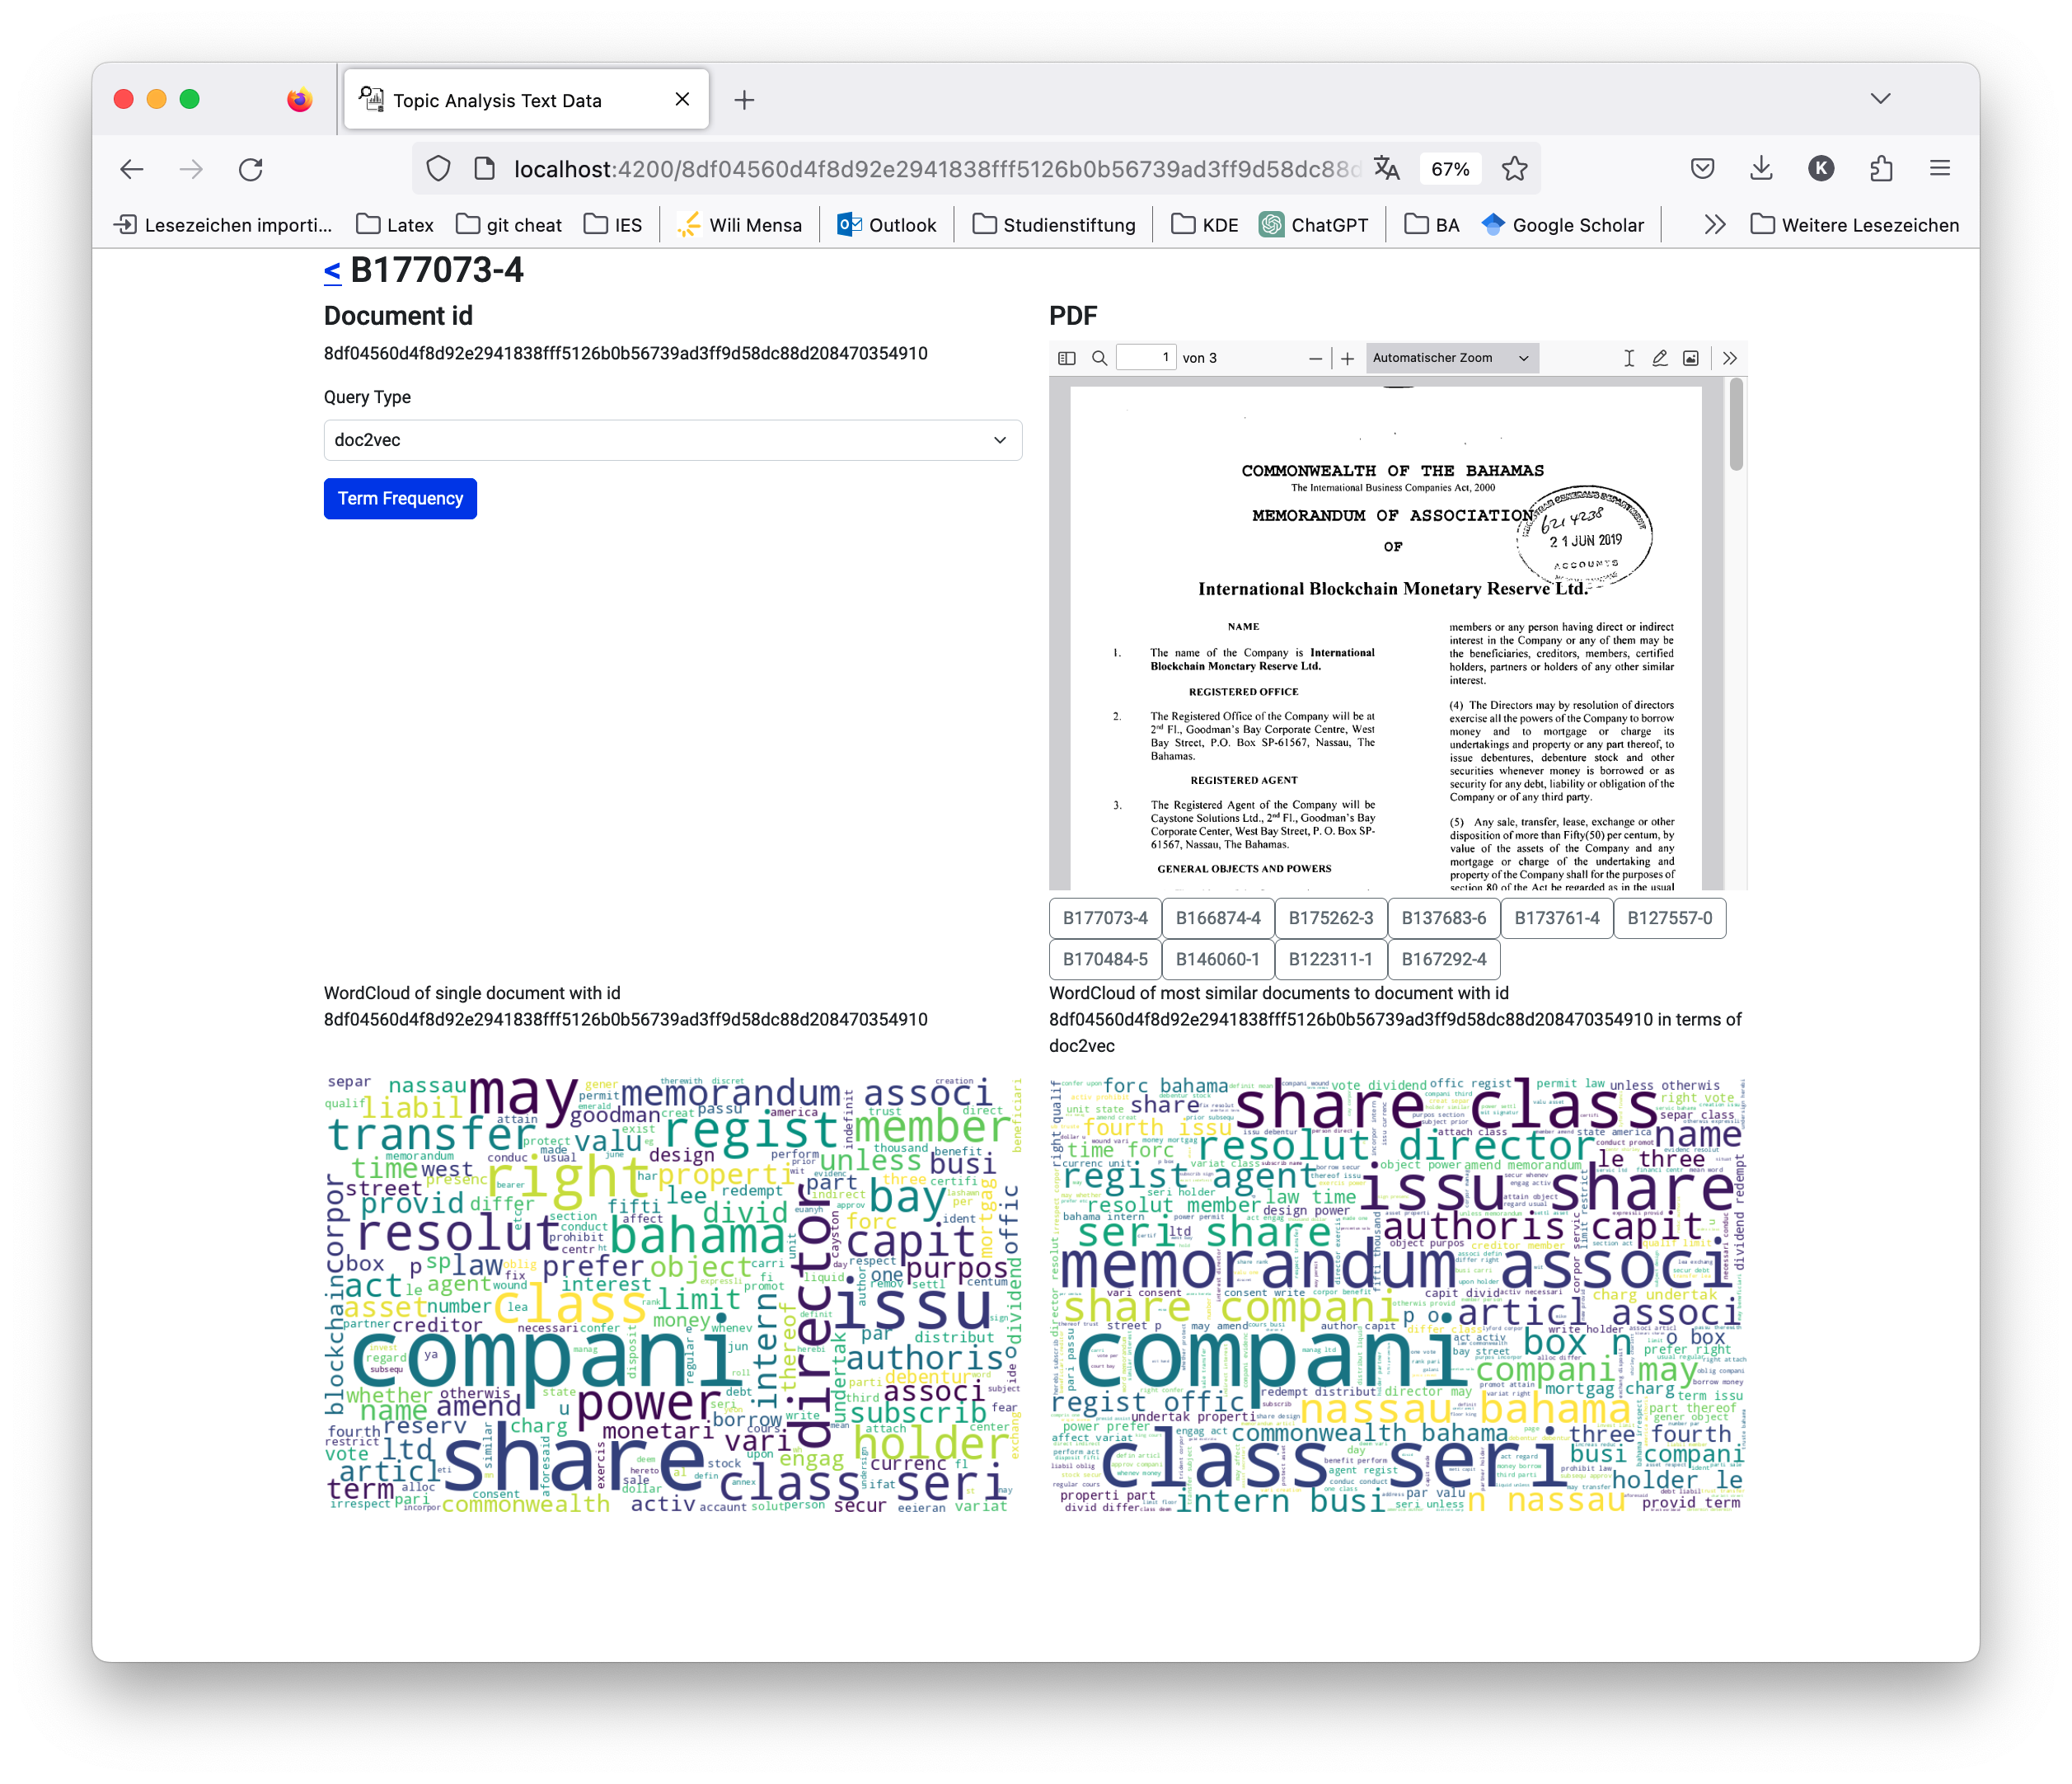
\includegraphics[width=0.6\textwidth]{images/UI/Home_detail.png}
    \caption{Detail component of the frontend.
    The chosen document is displayed, as well as its most similar documents in the database.
    WordClouds of the document and the most similar documents are displayed.
    }
    \label{fig:detail_comp}
\end{figure}


To change between the components, the routes have to be defined.
The routes are defined in the \texttt{app-routing.module.ts} file, as shown in \autoref{lst:angular_routing}.

\begin{listing}[htp]
    \begin{minted}{typescript}
        const routes: Routes = [
            { path: ':id', component: DocumentDetailComponent},
            { path: '', component: HomeComponent},
          ];
    \end{minted}
    \caption{Definition of routes in \angular{} in the app-routing.module.ts.
    }
    \label{lst:angular_routing}
\end{listing}